
\begin{figure}
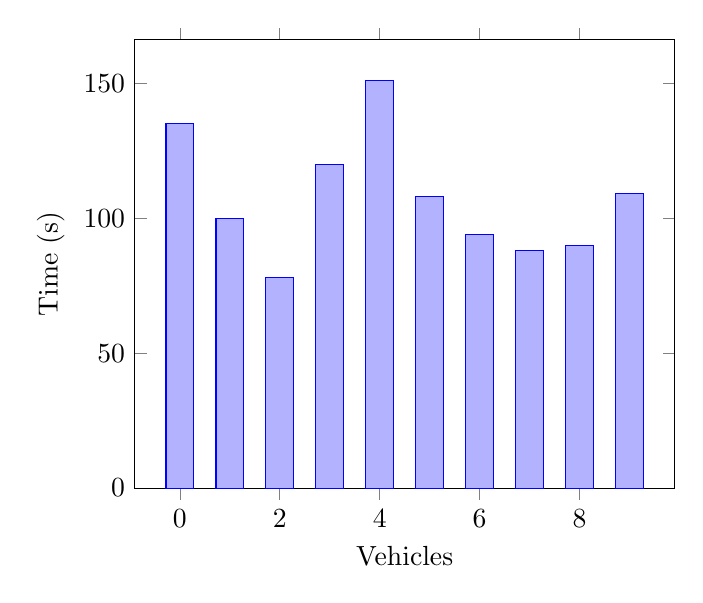
\begin{tikzpicture}
\begin{axis}[
legend style={anchor=west},
xlabel=Vehicles,
ylabel=Time (s),
ymin=0,
ybar,
]
\addplot coordinates {
(0, 135)
(1, 100)
(2, 78)
(3, 120)
(4, 151)
(5, 108)
(6, 94)
(7, 88)
(8, 90)
(9, 109)
};

\end{axis}
\end{tikzpicture}
\label{tik:0:14_V, 13_N, 13_N.-40, 11_N, 8_N, 7_N, 7_N.-60, 5_N, 4_N, 4_N.-60, 1_N}
\caption{0 percent diving with GSC on route $14_V, 13_N, 13_N.-40, 11_N, 8_N, 7_N, 7_N.-60, 5_N, 4_N, 4_N.-60, 1_N$}
\end{figure}
